% Options for packages loaded elsewhere
\PassOptionsToPackage{unicode}{hyperref}
\PassOptionsToPackage{hyphens}{url}
\documentclass[
]{article}
\usepackage{xcolor}
\usepackage[margin=1in]{geometry}
\usepackage{amsmath,amssymb}
\setcounter{secnumdepth}{-\maxdimen} % remove section numbering
\usepackage{iftex}
\ifPDFTeX
  \usepackage[T1]{fontenc}
  \usepackage[utf8]{inputenc}
  \usepackage{textcomp} % provide euro and other symbols
\else % if luatex or xetex
  \usepackage{unicode-math} % this also loads fontspec
  \defaultfontfeatures{Scale=MatchLowercase}
  \defaultfontfeatures[\rmfamily]{Ligatures=TeX,Scale=1}
\fi
\usepackage{lmodern}
\ifPDFTeX\else
  % xetex/luatex font selection
\fi
% Use upquote if available, for straight quotes in verbatim environments
\IfFileExists{upquote.sty}{\usepackage{upquote}}{}
\IfFileExists{microtype.sty}{% use microtype if available
  \usepackage[]{microtype}
  \UseMicrotypeSet[protrusion]{basicmath} % disable protrusion for tt fonts
}{}
\makeatletter
\@ifundefined{KOMAClassName}{% if non-KOMA class
  \IfFileExists{parskip.sty}{%
    \usepackage{parskip}
  }{% else
    \setlength{\parindent}{0pt}
    \setlength{\parskip}{6pt plus 2pt minus 1pt}}
}{% if KOMA class
  \KOMAoptions{parskip=half}}
\makeatother
\usepackage{color}
\usepackage{fancyvrb}
\newcommand{\VerbBar}{|}
\newcommand{\VERB}{\Verb[commandchars=\\\{\}]}
\DefineVerbatimEnvironment{Highlighting}{Verbatim}{commandchars=\\\{\}}
% Add ',fontsize=\small' for more characters per line
\usepackage{framed}
\definecolor{shadecolor}{RGB}{248,248,248}
\newenvironment{Shaded}{\begin{snugshade}}{\end{snugshade}}
\newcommand{\AlertTok}[1]{\textcolor[rgb]{0.94,0.16,0.16}{#1}}
\newcommand{\AnnotationTok}[1]{\textcolor[rgb]{0.56,0.35,0.01}{\textbf{\textit{#1}}}}
\newcommand{\AttributeTok}[1]{\textcolor[rgb]{0.13,0.29,0.53}{#1}}
\newcommand{\BaseNTok}[1]{\textcolor[rgb]{0.00,0.00,0.81}{#1}}
\newcommand{\BuiltInTok}[1]{#1}
\newcommand{\CharTok}[1]{\textcolor[rgb]{0.31,0.60,0.02}{#1}}
\newcommand{\CommentTok}[1]{\textcolor[rgb]{0.56,0.35,0.01}{\textit{#1}}}
\newcommand{\CommentVarTok}[1]{\textcolor[rgb]{0.56,0.35,0.01}{\textbf{\textit{#1}}}}
\newcommand{\ConstantTok}[1]{\textcolor[rgb]{0.56,0.35,0.01}{#1}}
\newcommand{\ControlFlowTok}[1]{\textcolor[rgb]{0.13,0.29,0.53}{\textbf{#1}}}
\newcommand{\DataTypeTok}[1]{\textcolor[rgb]{0.13,0.29,0.53}{#1}}
\newcommand{\DecValTok}[1]{\textcolor[rgb]{0.00,0.00,0.81}{#1}}
\newcommand{\DocumentationTok}[1]{\textcolor[rgb]{0.56,0.35,0.01}{\textbf{\textit{#1}}}}
\newcommand{\ErrorTok}[1]{\textcolor[rgb]{0.64,0.00,0.00}{\textbf{#1}}}
\newcommand{\ExtensionTok}[1]{#1}
\newcommand{\FloatTok}[1]{\textcolor[rgb]{0.00,0.00,0.81}{#1}}
\newcommand{\FunctionTok}[1]{\textcolor[rgb]{0.13,0.29,0.53}{\textbf{#1}}}
\newcommand{\ImportTok}[1]{#1}
\newcommand{\InformationTok}[1]{\textcolor[rgb]{0.56,0.35,0.01}{\textbf{\textit{#1}}}}
\newcommand{\KeywordTok}[1]{\textcolor[rgb]{0.13,0.29,0.53}{\textbf{#1}}}
\newcommand{\NormalTok}[1]{#1}
\newcommand{\OperatorTok}[1]{\textcolor[rgb]{0.81,0.36,0.00}{\textbf{#1}}}
\newcommand{\OtherTok}[1]{\textcolor[rgb]{0.56,0.35,0.01}{#1}}
\newcommand{\PreprocessorTok}[1]{\textcolor[rgb]{0.56,0.35,0.01}{\textit{#1}}}
\newcommand{\RegionMarkerTok}[1]{#1}
\newcommand{\SpecialCharTok}[1]{\textcolor[rgb]{0.81,0.36,0.00}{\textbf{#1}}}
\newcommand{\SpecialStringTok}[1]{\textcolor[rgb]{0.31,0.60,0.02}{#1}}
\newcommand{\StringTok}[1]{\textcolor[rgb]{0.31,0.60,0.02}{#1}}
\newcommand{\VariableTok}[1]{\textcolor[rgb]{0.00,0.00,0.00}{#1}}
\newcommand{\VerbatimStringTok}[1]{\textcolor[rgb]{0.31,0.60,0.02}{#1}}
\newcommand{\WarningTok}[1]{\textcolor[rgb]{0.56,0.35,0.01}{\textbf{\textit{#1}}}}
\usepackage{longtable,booktabs,array}
\newcounter{none} % for unnumbered tables
\usepackage{calc} % for calculating minipage widths
% Correct order of tables after \paragraph or \subparagraph
\usepackage{etoolbox}
\makeatletter
\patchcmd\longtable{\par}{\if@noskipsec\mbox{}\fi\par}{}{}
\makeatother
% Allow footnotes in longtable head/foot
\IfFileExists{footnotehyper.sty}{\usepackage{footnotehyper}}{\usepackage{footnote}}
\makesavenoteenv{longtable}
\usepackage{graphicx}
\makeatletter
\newsavebox\pandoc@box
\newcommand*\pandocbounded[1]{% scales image to fit in text height/width
  \sbox\pandoc@box{#1}%
  \Gscale@div\@tempa{\textheight}{\dimexpr\ht\pandoc@box+\dp\pandoc@box\relax}%
  \Gscale@div\@tempb{\linewidth}{\wd\pandoc@box}%
  \ifdim\@tempb\p@<\@tempa\p@\let\@tempa\@tempb\fi% select the smaller of both
  \ifdim\@tempa\p@<\p@\scalebox{\@tempa}{\usebox\pandoc@box}%
  \else\usebox{\pandoc@box}%
  \fi%
}
% Set default figure placement to htbp
\def\fps@figure{htbp}
\makeatother
\setlength{\emergencystretch}{3em} % prevent overfull lines
\providecommand{\tightlist}{%
  \setlength{\itemsep}{0pt}\setlength{\parskip}{0pt}}
\usepackage{booktabs}
\usepackage{longtable}
\usepackage{array}
\usepackage{multirow}
\usepackage{wrapfig}
\usepackage{float}
\usepackage{colortbl}
\usepackage{pdflscape}
\usepackage{tabularx}
\usepackage{xltabular}
\usepackage{threeparttable}
\usepackage{threeparttablex}
\usepackage[normalem]{ulem}
\usepackage{makecell}
\usepackage{xcolor}
\usepackage{bookmark}
\IfFileExists{xurl.sty}{\usepackage{xurl}}{} % add URL line breaks if available
\urlstyle{same}
\hypersetup{
  pdftitle={Unit 4.2: Numerical Methods},
  pdfauthor={Dr.~Manoj C. Patil},
  hidelinks,
  pdfcreator={LaTeX via pandoc}}

\title{Unit 4.2: Numerical Methods}
\author{Dr.~Manoj C. Patil}
\date{2026-09-19}

\begin{document}
\maketitle

\section{Learning Objectives}\label{learning-objectives}

By the end of this unit, a student should be able to

\begin{itemize}
\tightlist
\item
  explain why closed-form solutions to nonlinear equations and integrals
  are the exception rather than the rule in statistical practice,
  motivating numerical methods,
\item
  implement and prove the linear convergence of the bisection method for
  locating a root,
\item
  implement and prove the quadratic convergence of the Newton-Raphson
  method, and extend it to systems of nonlinear equations using the
  Jacobian matrix,
\item
  derive the trapezoidal and Simpson's rule quadrature formulas, their
  error terms, and their convergence rates,
\item
  implement all four methods in R and empirically verify their
  theoretical convergence rates,
\item
  recognize the role of these numerical methods within statistical
  computing, particularly maximum likelihood estimation and numerical
  integration of intractable expectations.
\end{itemize}

\section{Prerequisites}\label{prerequisites}

Students should be comfortable with

\begin{itemize}
\tightlist
\item
  single-variable and multivariable calculus, including Taylor's theorem
  with remainder and partial derivatives,
\item
  basic linear algebra, including matrix inversion and determinants of
  \(2\times2\) matrices,
\item
  the concept of a maximum likelihood estimator and the score equation,
\item
  R programming, including writing iterative loops and simple matrix
  operations.
\end{itemize}

\section{Introduction}\label{introduction}

Much of theoretical statistics is stated in a form that presumes an
equation can be solved, or an integral evaluated, exactly. The maximum
likelihood estimator is defined as the value that sets the score
function to zero; the sampling distribution of a statistic is often
described through an integral of a density; a quantile is defined
implicitly as the value \(x\) solving \(F(x)=u\). In practice,
closed-form solutions to these problems are the exception. The maximum
likelihood equations for all but the simplest models are nonlinear and
admit no algebraic solution; most integrals of interest in probability
and statistics --- even something as basic as the standard Normal
cumulative distribution function --- have no elementary antiderivative.
Numerical methods supply the machinery to solve such problems to any
desired accuracy using arithmetic operations alone.

This unit develops the two most fundamental families of numerical
methods used throughout statistical computing. \textbf{Root-finding
methods} --- the bisection method and the Newton-Raphson method ---
locate the value or values of \(x\) satisfying \(f(x)=0\), and extend
naturally to systems of nonlinear equations arising, for instance, from
multiparameter score equations. \textbf{Numerical integration methods}
--- the trapezoidal rule and Simpson's rule --- approximate a definite
integral using only evaluations of the integrand at a finite set of
points, and form the deterministic counterpart to the Monte Carlo
integration methods developed in Unit 4.3. The bisection method dates to
the ancient method of exhaustion and was formalized in the 19th century;
the Newton-Raphson method traces to Isaac Newton (1669) and Joseph
Raphson (1690); Simpson's rule, though named for Thomas Simpson (1743),
was known earlier to Johannes Kepler. Despite their age, these methods
remain the computational engines inside \texttt{optim()},
\texttt{nlm()}, \texttt{uniroot()}, and \texttt{integrate()} in R, and
inside virtually every statistical software package's maximum likelihood
fitting routines.

The practical importance of this material is immediate and pervasive:
fitting a generalized linear model, computing a profile likelihood
confidence interval, or evaluating the normalizing constant of a
posterior density all reduce, at some point, to root-finding or
numerical integration. Understanding how these building blocks work, and
their limitations, is essential to using statistical software correctly
and to diagnosing convergence failures when they occur.

\section{Intuition}\label{intuition}

Consider searching for a lost item along a long corridor, where a helper
can only tell you, at any point you ask, whether the item is to your
left or to your right. The most conservative strategy is to check the
midpoint of the corridor, learn which half the item is in, and repeat on
that half --- halving the search region at every step. This is exactly
the logic of the \textbf{bisection method}: given two points at which a
continuous function \(f\) has opposite signs, the Intermediate Value
Theorem guarantees a root lies between them, and evaluating the midpoint
and keeping whichever half still brackets a sign change halves the
uncertainty at every step, guaranteed, but never faster than that.

A sighted searcher who can also see how steeply the corridor's
brightness is changing could do better: standing at a point and
observing both the reading and its rate of change, they could
extrapolate --- assuming the trend continues in a straight line --- to
where the reading would hit zero, and jump there directly rather than
merely halving the interval. This is the idea behind the
\textbf{Newton-Raphson method}: at the current point \(x_n\),
approximate the function by its tangent line, and jump to where that
tangent line crosses zero. When the function is well approximated by its
tangent line near the root --- which a smooth function always is,
sufficiently close to a simple root --- this extrapolation converges far
faster than repeated halving.

A parallel intuition underlies numerical integration. The exact area
under a curve is unavailable in closed form, but the area under a
\emph{simple} curve --- a straight line, or a parabola --- passing
through a few known points of the true curve is easy to compute exactly.
The \textbf{trapezoidal rule} approximates the area under \(f\) on each
small sub-interval by the area under the straight line joining the two
endpoints; \textbf{Simpson's rule} does better by fitting a parabola
through three points at a time, exploiting the curvature information
that three points, rather than two, provide.

\begin{figure}

{\centering 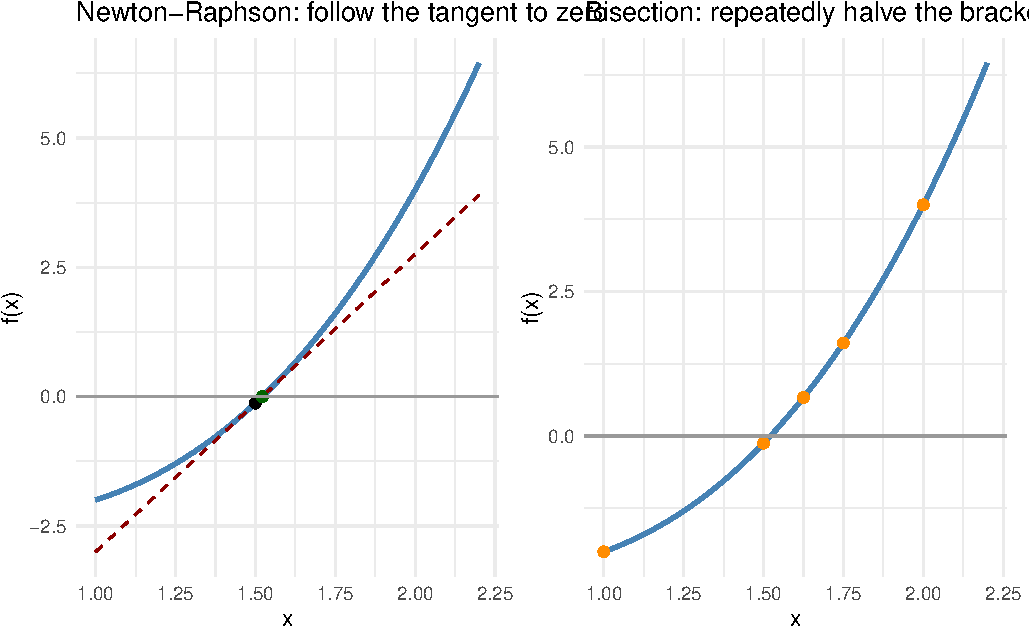
\includegraphics{04-02_Numerical_Methods_files/figure-latex/intuition-figure-1} 

}

\caption{Newton-Raphson (left) jumps to where the tangent line crosses zero, converging much faster near a smooth root than bisection's repeated halving (right).}\label{fig:intuition-figure}
\end{figure}

\section{Formal Definitions}\label{formal-definitions}

\subsection{The Root-Finding Problem}\label{the-root-finding-problem}

\textbf{Definition.} Given a continuous function \(f:\mathbb{R}\to
\mathbb{R}\), a \textbf{root} is a value \(r\) such that \(f(r)=0\). A
root \(r\) is \textbf{simple} if \(f'(r)\ne 0\).

\textbf{Definition (bracket).} An interval \([a,b]\) is said to
\textbf{bracket} a root of \(f\) if \(f(a)\) and \(f(b)\) have opposite
signs, i.e. \(f(a)f(b)<0\); by the Intermediate Value Theorem, a
continuous \(f\) then has at least one root in \((a,b)\).

\subsection{Systems of Nonlinear
Equations}\label{systems-of-nonlinear-equations}

\textbf{Definition.} For a vector-valued function
\(\mathbf F:\mathbb{R}^p\to\mathbb{R}^p\),
\(\mathbf F(\mathbf x) = (F_1(\mathbf x),\dots,F_p(\mathbf x))'\), a
\textbf{root} is a vector \(\mathbf r\) with \(\mathbf F(\mathbf r) =
\mathbf 0\). The \textbf{Jacobian matrix} of \(\mathbf F\) at
\(\mathbf x\) is

\[
J(\mathbf x) = \begin{pmatrix}
\dfrac{\partial F_1}{\partial x_1} & \cdots & \dfrac{\partial F_1}{\partial x_p} \\
\vdots & \ddots & \vdots \\
\dfrac{\partial F_p}{\partial x_1} & \cdots & \dfrac{\partial F_p}{\partial x_p}
\end{pmatrix}.
\tag{2.1}
\]

\subsection{Numerical Quadrature}\label{numerical-quadrature}

\textbf{Definition.} A \textbf{quadrature formula} approximates a
definite integral by a weighted sum of integrand values at prescribed
nodes,

\[
\int_a^b f(x)\,dx \;\approx\; \sum_{i=0}^{m} w_i\, f(x_i),
\tag{2.2}
\]

for nodes \(a=x_0<x_1<\cdots<x_m=b\) and weights \(w_i\) determined by
the specific rule. A quadrature rule has \textbf{degree of precision}
\(d\) if it integrates every polynomial of degree \(\le d\) exactly, and
fails to integrate some polynomial of degree \(d+1\) exactly.

\section{Theorems}\label{theorems}

\subsection{Theorem 2.1: Linear Convergence of the Bisection
Method}\label{theorem-2.1-linear-convergence-of-the-bisection-method}

\textbf{Statement.} Let \(f\) be continuous on \([a_0,b_0]\) with
\(f(a_0)f(b_0)<0\). The bisection method generates a sequence of
midpoints \(c_k\) satisfying

\[
|c_k - r| \le \frac{b_0-a_0}{2^{k+1}}
\tag{2.3}
\]

for some root \(r\in(a_0,b_0)\), for every \(k=0,1,2,\dots\).

\textbf{Assumptions.} \(f\) is continuous on \([a_0,b_0]\); only a sign
change is required, not differentiability.

\textbf{Proof.} By induction on \(k\), the bracket \([a_k,b_k]\)
maintained by the algorithm satisfies \(b_k-a_k = (b_0-a_0)/2^k\):
initially this holds for \(k=0\), and at each step the bracket width is
exactly halved by construction (the midpoint \(c_k=(a_k+b_k)/2\)
replaces whichever endpoint does not change sign with it, halving the
width). Since \(f(a_k)f(b_k)<0\) throughout (this sign-change property
is preserved by construction: the algorithm always keeps the
sub-interval on which the sign change persists), the Intermediate Value
Theorem guarantees a root \(r_k \in (a_k,b_k)\) at every step; because
the brackets are nested, all \(r_k\) coincide with a single root
\(r \in (a_0,b_0)\) common to every bracket. Since \(c_k\) is the
midpoint of \([a_k,b_k]\) and \(r\in[a_k,b_k]\),

\[
|c_k-r| \le \frac{b_k-a_k}{2} = \frac{b_0-a_0}{2^{k+1}},
\]

as claimed. \(\blacksquare\)

\textbf{Remarks.} The bound (2.3) holds unconditionally, with no
smoothness requirement on \(f\) beyond continuity; this robustness is
the bisection method's chief advantage, at the cost of convergence that
is always linear (each iteration gains a fixed number of correct bits,
not an increasing number).

\textbf{Examples.} A full worked example is given in Section 11.

\textbf{Applications.} Bisection is the standard fallback method inside
\texttt{uniroot()} in R, used whenever a robust (if slow) root-finder is
needed, for example to invert a monotone cumulative distribution
function numerically.

\subsection{Theorem 2.2: Quadratic Convergence of the Newton-Raphson
Method}\label{theorem-2.2-quadratic-convergence-of-the-newton-raphson-method}

\textbf{Statement.} Let \(r\) be a simple root of \(f\) (\(f(r)=0\),
\(f'(r)\ne0\)), with \(f\) twice continuously differentiable in a
neighbourhood of \(r\). If the Newton-Raphson iterates
\(x_{n+1} = x_n - f(x_n)/f'(x_n)\) are generated from a starting point
\(x_0\) sufficiently close to \(r\), then the errors \(e_n = r-x_n\)
satisfy

\[
e_{n+1} = -\frac{f''(\xi_n)}{2f'(x_n)}\, e_n^2
\tag{2.4}
\]

for some \(\xi_n\) between \(r\) and \(x_n\), and consequently there
exists a constant \(M\) (depending on bounds for \(f''\) and \(f'\) near
\(r\)) such that \(|e_{n+1}| \le M\, e_n^2\), i.e.~convergence is (at
least) quadratic.

\textbf{Assumptions.} \(f'(r)\ne 0\) (simple root); \(f''\) continuous
near \(r\); \(x_0\) close enough to \(r\) that all iterates remain in a
neighbourhood where \(f'\ne0\).

\textbf{Proof.} By Taylor's theorem with Lagrange remainder, expanding
\(f(r)\) about \(x_n\),

\[
0 = f(r) = f(x_n) + f'(x_n)(r-x_n) + \frac{f''(\xi_n)}{2}(r-x_n)^2
\]

for some \(\xi_n\) between \(x_n\) and \(r\). Dividing through by
\(f'(x_n)\) (non-zero for \(x_n\) close enough to \(r\), by continuity
of \(f'\) and \(f'(r)\ne0\)),

\[
\frac{f(x_n)}{f'(x_n)} + (r-x_n) = -\frac{f''(\xi_n)}{2f'(x_n)}(r-x_n)^2.
\]

Since \(x_{n+1} = x_n - f(x_n)/f'(x_n)\), the term \(f(x_n)/f'(x_n)\)
equals \(x_n - x_{n+1}\); substituting,

\[
(x_n-x_{n+1}) + (r-x_n) = -\frac{f''(\xi_n)}{2f'(x_n)}(r-x_n)^2
\;\Longrightarrow\;
r - x_{n+1} = -\frac{f''(\xi_n)}{2f'(x_n)}(r-x_n)^2,
\]

which is exactly (2.4). Taking \(M = \sup |f''|/\inf(2|f'|)\) over a
small neighbourhood of \(r\) (finite by continuity of \(f'\), \(f''\)
and \(f'(r)\ne0\)) gives \(|e_{n+1}| \le M e_n^2\). \(\blacksquare\)

\textbf{Remarks.} Quadratic convergence means that, once the iterates
are close enough to \(r\), the number of correct decimal digits
approximately \emph{doubles} at every iteration --- a dramatically
faster rate than bisection's fixed linear gain, as the numerical example
in Section 11 illustrates directly. The requirement that \(x_0\) be
``sufficiently close'' is essential: Newton-Raphson has no global
convergence guarantee analogous to bisection's, and can diverge, cycle,
or converge to an unintended root if started poorly or if \(f'(x_n)\)
comes close to zero during the iteration.

\textbf{Examples.} A full worked example is given in Section 11.

\textbf{Applications.} Newton-Raphson (and its generalization, Fisher
scoring, which replaces \(f'\) by its expectation) is the standard
algorithm used to solve the score equations of maximum likelihood
estimation for generalized linear models and countless other parametric
statistical models.

\section{Mathematical Derivations}\label{mathematical-derivations}

\subsection{Newton-Raphson for Systems of Nonlinear
Equations}\label{newton-raphson-for-systems-of-nonlinear-equations}

The scalar Newton-Raphson update \(x_{n+1}=x_n-f(x_n)/f'(x_n)\)
generalizes to a system \(\mathbf F(\mathbf x)=\mathbf 0\) by the same
tangent-line (now tangent-hyperplane) reasoning. Expanding \(\mathbf F\)
to first order about \(\mathbf x_n\),

\[
\mathbf 0 \approx \mathbf F(\mathbf x_n) + J(\mathbf x_n)(\mathbf x_{n+1}-\mathbf x_n),
\]

and solving for \(\mathbf x_{n+1}\) (assuming \(J(\mathbf x_n)\) is
invertible) gives the multivariate update

\[
\mathbf x_{n+1} = \mathbf x_n - J(\mathbf x_n)^{-1}\mathbf F(\mathbf x_n).
\tag{2.5}
\]

In practice, (2.5) is implemented not by explicitly inverting
\(J(\mathbf x_n)\) (computationally wasteful and numerically less
stable) but by solving the linear system
\(J(\mathbf x_n)\,\boldsymbol\delta_n = -\mathbf F(\mathbf x_n)\) for
the step \(\boldsymbol\delta_n\), and setting
\(\mathbf x_{n+1} = \mathbf x_n + \boldsymbol\delta_n\). Under the
analogous smoothness and non-singularity conditions to the scalar case,
the multivariate iteration also converges quadratically near a simple
root (a root at which \(J\) is non-singular).

\subsection{Derivation of the Trapezoidal Rule and Its
Error}\label{derivation-of-the-trapezoidal-rule-and-its-error}

On a single panel \([x_0,x_1]\) of width \(h=x_1-x_0\), the trapezoidal
rule replaces \(f\) by the straight line \(P_1\) interpolating
\((x_0,f(x_0))\) and \((x_1,f(x_1))\), giving

\[
\int_{x_0}^{x_1} f(x)\,dx \approx \int_{x_0}^{x_1} P_1(x)\,dx
= \frac{h}{2}\bigl(f(x_0)+f(x_1)\bigr).
\tag{2.6}
\]

The standard linear interpolation error formula gives
\(f(x)-P_1(x) = \tfrac12 f''(\eta(x))(x-x_0)(x-x_1)\) for some
\(\eta(x)\) between \(x_0\) and \(x_1\) (a consequence of Rolle's
theorem applied to the interpolation remainder; see Burden \& Faires,
2011, Thm. 3.3). Since \((x-x_0)(x-x_1)\le 0\) throughout \([x_0,x_1]\),
the weighted mean value theorem for integrals gives, for some
\(\xi\in(x_0,x_1)\),

\[
\int_{x_0}^{x_1} \bigl[f(x)-P_1(x)\bigr]dx
= \frac{f''(\xi)}{2}\int_{x_0}^{x_1}(x-x_0)(x-x_1)\,dx
= \frac{f''(\xi)}{2}\left(-\frac{h^3}{6}\right) = -\frac{h^3}{12}f''(\xi),
\tag{2.7}
\]

using the standard result
\(\int_{x_0}^{x_1}(x-x_0)(x-x_1)\,dx = -h^3/6\) (verified directly by
substitution \(u=x-x_0\):
\(\int_0^h u(u-h)\,du = \bigl[u^3/3-hu^2/2\bigr]_0^h
= h^3/3-h^3/2=-h^3/6\)). Summing (2.7) over \(n\) panels of a composite
rule and applying a further mean value argument to the sum of the
per-panel errors (each proportional to \(h^3f''(\xi_i)\), summed and
recognized as an \(O(h)\)-spaced Riemann-type sum) gives the composite
trapezoidal error

\[
E_{\text{trap}} = -\frac{(b-a)h^2}{12} f''(\xi), \qquad \xi\in(a,b),
\tag{2.8}
\]

confirming that the composite trapezoidal rule has error \(O(h^2)\).

\subsection{Derivation of Simpson's Rule and Its
Error}\label{derivation-of-simpsons-rule-and-its-error}

Simpson's rule approximates the integral over a panel \([x_0,x_2]\) of
width \(2h\), with midpoint \(x_1=x_0+h\), by fitting a quadratic
through the three points. Writing \(m=x_1\) and expanding both the exact
integral and the quadrature rule in a Taylor series about \(m\) makes
the derivation self-contained. Using
\(f(x)=f(m)+f'(m)(x-m)+\tfrac12f''(m)(x-m)^2+\tfrac16f'''(m)(x-m)^3
+\tfrac{1}{24}f''''(m)(x-m)^4+\cdots\) and integrating term by term over
\([m-h,m+h]\) (odd-power terms vanish by symmetry),

\[
\int_{m-h}^{m+h} f(x)\,dx = 2h f(m) + \frac{h^3}{3}f''(m)
+ \frac{h^5}{60}f''''(m) + O(h^7).
\tag{2.9}
\]

For the quadrature side, Simpson's rule is
\(S = \tfrac{h}{3}\bigl[f(m-h)+4f(m)+f(m+h)\bigr]\); Taylor-expanding
\(f(m-h)\) and \(f(m+h)\) and adding (again the odd terms cancel),
\(f(m-h)+f(m+h) = 2f(m)+h^2f''(m)+\tfrac{h^4}{12}f''''(m)+O(h^6)\), so

\[
S = \frac{h}{3}\Bigl[6f(m) + h^2 f''(m) + \frac{h^4}{12}f''''(m)\Bigr] + O(h^7)
= 2hf(m) + \frac{h^3}{3}f''(m) + \frac{h^5}{36}f''''(m) + O(h^7).
\tag{2.10}
\]

Subtracting (2.10) from (2.9), the \(f(m)\) and \(f''(m)\) terms cancel
exactly, leaving

\[
E_{\text{Simpson, panel}} = \Bigl(\frac{1}{60}-\frac{1}{36}\Bigr)h^5 f''''(m) + O(h^7)
= -\frac{h^5}{90}f''''(\xi)
\tag{2.11}
\]

for some \(\xi\) near \(m\) (replacing \(f''''(m)\) by \(f''''(\xi)\)
via the mean value theorem to absorb the \(O(h^7)\) remainder). Summing
over \(n/2\) panels of a composite rule (an even number \(n\) of
sub-intervals is required) gives the standard composite Simpson error

\[
E_{\text{Simpson}} = -\frac{(b-a)h^4}{180} f''''(\xi), \qquad \xi\in(a,b),
\tag{2.12}
\]

showing the composite Simpson's rule has error \(O(h^4)\) --- two full
orders better than the trapezoidal rule's \(O(h^2)\) for a comparable
number of function evaluations, at the cost of requiring an even number
of sub-intervals and one additional order of smoothness (\(f''''\)
rather than \(f''\)).

\section{Algorithms}\label{algorithms}

\subsection{Algorithm 2.1: Bisection
Method}\label{algorithm-2.1-bisection-method}

\textbf{Purpose.} Locate a root of \(f\) within a bracket \([a,b]\),
with a guaranteed, if slow, rate of convergence.

\textbf{Input.} Function \(f\); bracket \([a,b]\) with \(f(a)f(b)<0\);
tolerance \(\varepsilon\).

\textbf{Output.} An approximate root \(c\) with \(|c-r| < \varepsilon\).

\textbf{Step-by-step procedure.}

\begin{enumerate}
\def\labelenumi{\arabic{enumi}.}
\tightlist
\item
  While \((b-a)/2 > \varepsilon\):

  \begin{enumerate}
  \def\labelenumii{(\alph{enumii})}
  \tightlist
  \item
    compute \(c=(a+b)/2\);
  \item
    if \(f(a)f(c) < 0\), set \(b=c\); otherwise set \(a=c\).
  \end{enumerate}
\item
  Return \(c=(a+b)/2\).
\end{enumerate}

\textbf{Pseudo-code.}

\begin{verbatim}
Algorithm: Bisection Method
Input:  f, a, b (with f(a)*f(b) < 0), epsilon
Output: approximate root c

1. While (b - a) / 2 > epsilon:
       c <- (a + b) / 2
       If f(a) * f(c) < 0:
           b <- c
       Else:
           a <- c
2. Return (a + b) / 2
\end{verbatim}

\textbf{Flowchart description.} Start; check the width of the bracket
against the tolerance; if too wide, compute the midpoint, evaluate the
function there, and replace whichever endpoint shares its sign with the
midpoint; repeat; once the bracket is narrow enough, return the
midpoint; end.

\textbf{Complexity.} \(O(\log_2((b-a)/\varepsilon))\) iterations, each
costing one function evaluation, by Theorem 2.1.

\textbf{Practical considerations.} Bisection requires only a valid
initial bracket, and always converges for a continuous function once one
is found; it is the natural fallback when Newton-Raphson fails to
converge or when derivatives of \(f\) are unavailable or unreliable.

\subsection{Algorithm 2.2: Newton-Raphson
Method}\label{algorithm-2.2-newton-raphson-method}

\textbf{Purpose.} Locate a root of \(f\) rapidly, using derivative
information, near a good starting guess.

\textbf{Input.} Function \(f\) and its derivative \(f'\); starting point
\(x_0\); tolerance \(\varepsilon\); maximum iterations \(N\).

\textbf{Output.} An approximate root \(x_n\).

\textbf{Step-by-step procedure.}

\begin{enumerate}
\def\labelenumi{\arabic{enumi}.}
\tightlist
\item
  For \(n=0,1,2,\dots\) until \(|x_{n+1}-x_n|<\varepsilon\) or \(n=N\):
  compute \(x_{n+1} = x_n - f(x_n)/f'(x_n)\).
\item
  Return the final iterate.
\end{enumerate}

\textbf{Pseudo-code.}

\begin{verbatim}
Algorithm: Newton-Raphson Method
Input:  f, f_prime, x0, epsilon, N
Output: approximate root x

1. x <- x0
2. For n = 1 to N:
       x_new <- x - f(x) / f_prime(x)
       If |x_new - x| < epsilon:
           Return x_new
       x <- x_new
3. Return x  (or report non-convergence)
\end{verbatim}

\textbf{Flowchart description.} Start; evaluate \(f\) and \(f'\) at the
current iterate; compute the tangent-line intercept as the new iterate;
check for convergence; if not converged and the iteration budget
remains, repeat; end.

\textbf{Complexity.} Under quadratic convergence (Theorem 2.2), the
number of iterations to reach tolerance \(\varepsilon\), once in the
basin of quadratic convergence, is \(O(\log\log(1/\varepsilon))\) ---
dramatically fewer than bisection's \(O(\log(1/\varepsilon))\) --- but
each iteration requires evaluating both \(f\) and \(f'\).

\textbf{Practical considerations.} Newton-Raphson can fail --- diverge,
cycle, or converge to the wrong root --- if \(x_0\) is poorly chosen or
\(f'(x_n)\) is close to zero at some iterate; a common safeguard is to
combine Newton-Raphson with a bisection fallback (as \texttt{uniroot()}
and professional root-finders do) to retain global reliability while
benefiting from Newton's local speed.

\subsection{Algorithm 2.3: Newton-Raphson for Systems of Nonlinear
Equations}\label{algorithm-2.3-newton-raphson-for-systems-of-nonlinear-equations}

\textbf{Purpose.} Solve \(\mathbf F(\mathbf x)=\mathbf 0\) for a
vector-valued \(\mathbf F\), generalizing Algorithm 2.2 using (2.5).

\textbf{Input.} Function \(\mathbf F\) and its Jacobian \(J\); starting
vector \(\mathbf x_0\); tolerance \(\varepsilon\); maximum iterations
\(N\).

\textbf{Output.} An approximate root \(\mathbf x_n\).

\textbf{Step-by-step procedure.}

\begin{enumerate}
\def\labelenumi{\arabic{enumi}.}
\tightlist
\item
  For \(n=0,1,2,\dots\) until \(\|\mathbf x_{n+1}-\mathbf x_n\|<
  \varepsilon\) or \(n=N\): solve the linear system
  \(J(\mathbf x_n)\boldsymbol\delta_n = -\mathbf F(\mathbf x_n)\) for
  \(\boldsymbol\delta_n\); set \(\mathbf x_{n+1} = \mathbf x_n +
  \boldsymbol\delta_n\).
\item
  Return the final iterate.
\end{enumerate}

\textbf{Pseudo-code.}

\begin{verbatim}
Algorithm: Newton-Raphson for Systems
Input:  F, J, x0, epsilon, N
Output: approximate root vector x

1. x <- x0
2. For n = 1 to N:
       delta <- solve( J(x), -F(x) )
       x_new <- x + delta
       If norm(x_new - x) < epsilon:
           Return x_new
       x <- x_new
3. Return x  (or report non-convergence)
\end{verbatim}

\textbf{Flowchart description.} Start; evaluate \(\mathbf F\) and \(J\)
at the current vector iterate; solve the resulting linear system for the
step; update the iterate; check convergence in norm; repeat if not
converged; end.

\textbf{Complexity.} Each iteration costs \(O(p^3)\) for solving the
\(p\times p\) linear system (via Gaussian elimination or LU
decomposition), in addition to the cost of evaluating \(\mathbf F\) and
\(J\); the number of iterations required is again \(O(\log\log(1/
\varepsilon))\) near a simple root under the multivariate analogue of
Theorem 2.2.

\textbf{Practical considerations.} A singular or near-singular Jacobian
at any iterate causes the linear solve to fail or become numerically
unstable; monitoring the condition number of \(J(\mathbf x_n)\), or
adding a small ridge term when necessary, is standard practice in
production implementations (as in the Levenberg-Marquardt modification
used for nonlinear least squares).

\subsection{Algorithm 2.4: Composite Trapezoidal and Simpson's
Rules}\label{algorithm-2.4-composite-trapezoidal-and-simpsons-rules}

\textbf{Purpose.} Approximate \(\int_a^b f(x)\,dx\) using evenly spaced
function evaluations.

\textbf{Input.} Function \(f\); interval \([a,b]\); number of
sub-intervals \(n\) (even, for Simpson's rule).

\textbf{Output.} Approximate integral value.

\textbf{Step-by-step procedure (Trapezoidal).}

\begin{enumerate}
\def\labelenumi{\arabic{enumi}.}
\tightlist
\item
  Set \(h=(b-a)/n\) and \(x_i = a+ih\), \(i=0,\dots,n\).
\item
  Compute
  \(T = \dfrac{h}{2}\Bigl[f(x_0) + 2\sum_{i=1}^{n-1}f(x_i) + f(x_n)\Bigr]\).
\end{enumerate}

\textbf{Step-by-step procedure (Simpson's, \(n\) even).}

\begin{enumerate}
\def\labelenumi{\arabic{enumi}.}
\tightlist
\item
  Set \(h=(b-a)/n\) and \(x_i=a+ih\), \(i=0,\dots,n\).
\item
  Compute
  \(S = \dfrac{h}{3}\Bigl[f(x_0)+4\!\!\sum_{i\ \text{odd}}\!\!f(x_i)
  +2\!\!\sum_{i\ \text{even},\,0<i<n}\!\!f(x_i)+f(x_n)\Bigr]\).
\end{enumerate}

\textbf{Pseudo-code.}

\begin{verbatim}
Algorithm: Composite Trapezoidal / Simpson's Rule
Input:  f, a, b, n
Output: approximate integral

1. h <- (b - a) / n
2. x[0..n] <- a + i * h  for i = 0..n
3. Trapezoidal:
       T <- h/2 * ( f(x[0]) + 2*sum(f(x[1..n-1])) + f(x[n]) )
4. Simpson (n even):
       S <- h/3 * ( f(x[0]) + 4*sum(f(x[odd i])) + 2*sum(f(x[even i, interior])) + f(x[n]) )
5. Return T (or S)
\end{verbatim}

\textbf{Flowchart description.} Start; partition \([a,b]\) into \(n\)
equal sub-intervals; evaluate \(f\) at every node; combine the values
with the prescribed weights (uniform for the endpoints and alternating
4-2-4-2 weights for Simpson's interior nodes); return the weighted sum;
end.

\textbf{Complexity.} \(O(n)\) function evaluations for both rules;
Simpson's rule achieves \(O(h^4)\) accuracy against the trapezoidal
rule's \(O(h^2)\) for the same \(n\) (hence the same computational
cost), making it strictly preferable whenever \(f''''\) is well behaved.

\textbf{Practical considerations.} Both rules degrade for integrands
with sharp peaks, discontinuities, or singularities within \([a,b]\);
adaptive quadrature (as implemented in R's \texttt{integrate()}), which
concentrates evaluation points where the integrand varies most rapidly,
should be preferred for such integrands over a fixed-\(n\) composite
rule.

\section{R Programming}\label{r-programming}

\begin{Shaded}
\begin{Highlighting}[]
\FunctionTok{set.seed}\NormalTok{(}\DecValTok{123}\NormalTok{)}

\CommentTok{\#\textquotesingle{} Bisection method for root{-}finding}
\CommentTok{\#\textquotesingle{}}
\CommentTok{\#\textquotesingle{} Purpose: implements Algorithm 2.1.}
\CommentTok{\#\textquotesingle{}}
\CommentTok{\#\textquotesingle{} Arguments:}
\CommentTok{\#\textquotesingle{}   target\_function   function f for which a root is sought}
\CommentTok{\#\textquotesingle{}   lower\_bound       left endpoint of the bracket}
\CommentTok{\#\textquotesingle{}   upper\_bound       right endpoint of the bracket}
\CommentTok{\#\textquotesingle{}   tolerance         stopping tolerance on the bracket width}
\CommentTok{\#\textquotesingle{}}
\CommentTok{\#\textquotesingle{} Returns:}
\CommentTok{\#\textquotesingle{}   a list with the approximate root and the iteration history}
\CommentTok{\#\textquotesingle{}}
\CommentTok{\#\textquotesingle{} Example:}
\CommentTok{\#\textquotesingle{}   bisection\_method(function(x) x\^{}3 {-} x {-} 2, 1, 2, 1e{-}8)}
\NormalTok{bisection\_method }\OtherTok{\textless{}{-}} \ControlFlowTok{function}\NormalTok{(target\_function, lower\_bound, upper\_bound, }\AttributeTok{tolerance =} \FloatTok{1e{-}8}\NormalTok{) \{}
  \ControlFlowTok{if}\NormalTok{ (}\FunctionTok{target\_function}\NormalTok{(lower\_bound) }\SpecialCharTok{*} \FunctionTok{target\_function}\NormalTok{(upper\_bound) }\SpecialCharTok{\textgreater{}=} \DecValTok{0}\NormalTok{) \{}
    \FunctionTok{stop}\NormalTok{(}\StringTok{"The supplied interval does not bracket a root."}\NormalTok{)}
\NormalTok{  \}}

\NormalTok{  iteration\_history }\OtherTok{\textless{}{-}} \FunctionTok{numeric}\NormalTok{(}\DecValTok{0}\NormalTok{)}
  \ControlFlowTok{while}\NormalTok{ ((upper\_bound }\SpecialCharTok{{-}}\NormalTok{ lower\_bound) }\SpecialCharTok{/} \DecValTok{2} \SpecialCharTok{\textgreater{}}\NormalTok{ tolerance) \{}
\NormalTok{    midpoint }\OtherTok{\textless{}{-}}\NormalTok{ (lower\_bound }\SpecialCharTok{+}\NormalTok{ upper\_bound) }\SpecialCharTok{/} \DecValTok{2}
\NormalTok{    iteration\_history }\OtherTok{\textless{}{-}} \FunctionTok{c}\NormalTok{(iteration\_history, midpoint)}

    \ControlFlowTok{if}\NormalTok{ (}\FunctionTok{target\_function}\NormalTok{(lower\_bound) }\SpecialCharTok{*} \FunctionTok{target\_function}\NormalTok{(midpoint) }\SpecialCharTok{\textless{}} \DecValTok{0}\NormalTok{) \{}
\NormalTok{      upper\_bound }\OtherTok{\textless{}{-}}\NormalTok{ midpoint}
\NormalTok{    \} }\ControlFlowTok{else}\NormalTok{ \{}
\NormalTok{      lower\_bound }\OtherTok{\textless{}{-}}\NormalTok{ midpoint}
\NormalTok{    \}}
\NormalTok{  \}}

  \FunctionTok{list}\NormalTok{(}\AttributeTok{root =}\NormalTok{ (lower\_bound }\SpecialCharTok{+}\NormalTok{ upper\_bound) }\SpecialCharTok{/} \DecValTok{2}\NormalTok{, }\AttributeTok{history =}\NormalTok{ iteration\_history)}
\NormalTok{\}}

\CommentTok{\#\textquotesingle{} Newton{-}Raphson method for root{-}finding}
\CommentTok{\#\textquotesingle{}}
\CommentTok{\#\textquotesingle{} Purpose: implements Algorithm 2.2.}
\CommentTok{\#\textquotesingle{}}
\CommentTok{\#\textquotesingle{} Arguments:}
\CommentTok{\#\textquotesingle{}   target\_function     function f}
\CommentTok{\#\textquotesingle{}   target\_derivative   function f\textquotesingle{}}
\CommentTok{\#\textquotesingle{}   starting\_point      initial guess x0}
\CommentTok{\#\textquotesingle{}   tolerance           stopping tolerance on successive iterates}
\CommentTok{\#\textquotesingle{}   max\_iterations      maximum number of iterations}
\CommentTok{\#\textquotesingle{}}
\CommentTok{\#\textquotesingle{} Returns:}
\CommentTok{\#\textquotesingle{}   a list with the approximate root and the iteration history}
\CommentTok{\#\textquotesingle{}}
\CommentTok{\#\textquotesingle{} Example:}
\CommentTok{\#\textquotesingle{}   newton\_raphson\_method(}
\CommentTok{\#\textquotesingle{}     function(x) x\^{}3 {-} x {-} 2, function(x) 3 * x\^{}2 {-} 1, 1.5, 1e{-}10}
\CommentTok{\#\textquotesingle{}   )}
\NormalTok{newton\_raphson\_method }\OtherTok{\textless{}{-}} \ControlFlowTok{function}\NormalTok{(target\_function, target\_derivative, starting\_point,}
                                   \AttributeTok{tolerance =} \FloatTok{1e{-}10}\NormalTok{, }\AttributeTok{max\_iterations =} \DecValTok{100}\NormalTok{) \{}
\NormalTok{  current\_point }\OtherTok{\textless{}{-}}\NormalTok{ starting\_point}
\NormalTok{  iteration\_history }\OtherTok{\textless{}{-}}\NormalTok{ current\_point}

  \ControlFlowTok{for}\NormalTok{ (iteration }\ControlFlowTok{in} \FunctionTok{seq\_len}\NormalTok{(max\_iterations)) \{}
\NormalTok{    next\_point }\OtherTok{\textless{}{-}}\NormalTok{ current\_point }\SpecialCharTok{{-}} \FunctionTok{target\_function}\NormalTok{(current\_point) }\SpecialCharTok{/} \FunctionTok{target\_derivative}\NormalTok{(current\_point)}
\NormalTok{    iteration\_history }\OtherTok{\textless{}{-}} \FunctionTok{c}\NormalTok{(iteration\_history, next\_point)}

    \ControlFlowTok{if}\NormalTok{ (}\FunctionTok{abs}\NormalTok{(next\_point }\SpecialCharTok{{-}}\NormalTok{ current\_point) }\SpecialCharTok{\textless{}}\NormalTok{ tolerance) \{}
      \FunctionTok{return}\NormalTok{(}\FunctionTok{list}\NormalTok{(}\AttributeTok{root =}\NormalTok{ next\_point, }\AttributeTok{history =}\NormalTok{ iteration\_history))}
\NormalTok{    \}}
\NormalTok{    current\_point }\OtherTok{\textless{}{-}}\NormalTok{ next\_point}
\NormalTok{  \}}

  \FunctionTok{list}\NormalTok{(}\AttributeTok{root =}\NormalTok{ current\_point, }\AttributeTok{history =}\NormalTok{ iteration\_history)}
\NormalTok{\}}

\CommentTok{\#\textquotesingle{} Newton{-}Raphson method for systems of nonlinear equations}
\CommentTok{\#\textquotesingle{}}
\CommentTok{\#\textquotesingle{} Purpose: implements Algorithm 2.3.}
\CommentTok{\#\textquotesingle{}}
\CommentTok{\#\textquotesingle{} Arguments:}
\CommentTok{\#\textquotesingle{}   system\_function     function returning the vector F(x)}
\CommentTok{\#\textquotesingle{}   jacobian\_function    function returning the Jacobian matrix J(x)}
\CommentTok{\#\textquotesingle{}   starting\_vector      initial guess x0}
\CommentTok{\#\textquotesingle{}   tolerance            stopping tolerance on the step norm}
\CommentTok{\#\textquotesingle{}   max\_iterations       maximum number of iterations}
\CommentTok{\#\textquotesingle{}}
\CommentTok{\#\textquotesingle{} Returns:}
\CommentTok{\#\textquotesingle{}   a list with the approximate root vector and the iteration history}
\CommentTok{\#\textquotesingle{}}
\CommentTok{\#\textquotesingle{} Example:}
\CommentTok{\#\textquotesingle{}   newton\_raphson\_system(}
\CommentTok{\#\textquotesingle{}     function(v) c(v[1]\^{}2 + v[2]\^{}2 {-} 4, v[1] * v[2] {-} 1),}
\CommentTok{\#\textquotesingle{}     function(v) matrix(c(2 * v[1], v[2], 2 * v[2], v[1]), nrow = 2),}
\CommentTok{\#\textquotesingle{}     c(1.8, 0.6)}
\CommentTok{\#\textquotesingle{}   )}
\NormalTok{newton\_raphson\_system }\OtherTok{\textless{}{-}} \ControlFlowTok{function}\NormalTok{(system\_function, jacobian\_function, starting\_vector,}
                                   \AttributeTok{tolerance =} \FloatTok{1e{-}10}\NormalTok{, }\AttributeTok{max\_iterations =} \DecValTok{100}\NormalTok{) \{}
\NormalTok{  current\_vector }\OtherTok{\textless{}{-}}\NormalTok{ starting\_vector}
\NormalTok{  iteration\_history }\OtherTok{\textless{}{-}} \FunctionTok{list}\NormalTok{(current\_vector)}

  \ControlFlowTok{for}\NormalTok{ (iteration }\ControlFlowTok{in} \FunctionTok{seq\_len}\NormalTok{(max\_iterations)) \{}
\NormalTok{    step\_vector }\OtherTok{\textless{}{-}} \FunctionTok{solve}\NormalTok{(}\FunctionTok{jacobian\_function}\NormalTok{(current\_vector), }\SpecialCharTok{{-}}\FunctionTok{system\_function}\NormalTok{(current\_vector))}
\NormalTok{    next\_vector }\OtherTok{\textless{}{-}}\NormalTok{ current\_vector }\SpecialCharTok{+}\NormalTok{ step\_vector}
\NormalTok{    iteration\_history[[iteration }\SpecialCharTok{+} \DecValTok{1}\NormalTok{]] }\OtherTok{\textless{}{-}}\NormalTok{ next\_vector}

    \ControlFlowTok{if}\NormalTok{ (}\FunctionTok{sqrt}\NormalTok{(}\FunctionTok{sum}\NormalTok{((next\_vector }\SpecialCharTok{{-}}\NormalTok{ current\_vector)}\SpecialCharTok{\^{}}\DecValTok{2}\NormalTok{)) }\SpecialCharTok{\textless{}}\NormalTok{ tolerance) \{}
      \FunctionTok{return}\NormalTok{(}\FunctionTok{list}\NormalTok{(}\AttributeTok{root =}\NormalTok{ next\_vector, }\AttributeTok{history =}\NormalTok{ iteration\_history))}
\NormalTok{    \}}
\NormalTok{    current\_vector }\OtherTok{\textless{}{-}}\NormalTok{ next\_vector}
\NormalTok{  \}}

  \FunctionTok{list}\NormalTok{(}\AttributeTok{root =}\NormalTok{ current\_vector, }\AttributeTok{history =}\NormalTok{ iteration\_history)}
\NormalTok{\}}

\CommentTok{\#\textquotesingle{} Composite trapezoidal rule}
\CommentTok{\#\textquotesingle{}}
\CommentTok{\#\textquotesingle{} Purpose: implements the trapezoidal part of Algorithm 2.4.}
\CommentTok{\#\textquotesingle{}}
\CommentTok{\#\textquotesingle{} Arguments:}
\CommentTok{\#\textquotesingle{}   integrand\_function   function to integrate}
\CommentTok{\#\textquotesingle{}   lower\_limit          lower limit of integration}
\CommentTok{\#\textquotesingle{}   upper\_limit          upper limit of integration}
\CommentTok{\#\textquotesingle{}   number\_of\_intervals  number of sub{-}intervals}
\CommentTok{\#\textquotesingle{}}
\CommentTok{\#\textquotesingle{} Returns:}
\CommentTok{\#\textquotesingle{}   the approximate integral (numeric scalar)}
\CommentTok{\#\textquotesingle{}}
\CommentTok{\#\textquotesingle{} Example:}
\CommentTok{\#\textquotesingle{}   trapezoidal\_rule(function(x) x\^{}2, 0, 2, 4)}
\NormalTok{trapezoidal\_rule }\OtherTok{\textless{}{-}} \ControlFlowTok{function}\NormalTok{(integrand\_function, lower\_limit, upper\_limit, number\_of\_intervals) \{}
\NormalTok{  step\_size }\OtherTok{\textless{}{-}}\NormalTok{ (upper\_limit }\SpecialCharTok{{-}}\NormalTok{ lower\_limit) }\SpecialCharTok{/}\NormalTok{ number\_of\_intervals}
\NormalTok{  grid\_points }\OtherTok{\textless{}{-}}\NormalTok{ lower\_limit }\SpecialCharTok{+}\NormalTok{ (}\DecValTok{0}\SpecialCharTok{:}\NormalTok{number\_of\_intervals) }\SpecialCharTok{*}\NormalTok{ step\_size}
\NormalTok{  function\_values }\OtherTok{\textless{}{-}} \FunctionTok{integrand\_function}\NormalTok{(grid\_points)}

\NormalTok{  step\_size }\SpecialCharTok{/} \DecValTok{2} \SpecialCharTok{*}\NormalTok{ (function\_values[}\DecValTok{1}\NormalTok{] }\SpecialCharTok{+} \DecValTok{2} \SpecialCharTok{*} \FunctionTok{sum}\NormalTok{(function\_values[}\DecValTok{2}\SpecialCharTok{:}\NormalTok{number\_of\_intervals]) }\SpecialCharTok{+}
\NormalTok{    function\_values[number\_of\_intervals }\SpecialCharTok{+} \DecValTok{1}\NormalTok{])}
\NormalTok{\}}

\CommentTok{\#\textquotesingle{} Composite Simpson\textquotesingle{}s rule}
\CommentTok{\#\textquotesingle{}}
\CommentTok{\#\textquotesingle{} Purpose: implements the Simpson\textquotesingle{}s part of Algorithm 2.4.}
\CommentTok{\#\textquotesingle{}}
\CommentTok{\#\textquotesingle{} Arguments:}
\CommentTok{\#\textquotesingle{}   integrand\_function   function to integrate}
\CommentTok{\#\textquotesingle{}   lower\_limit          lower limit of integration}
\CommentTok{\#\textquotesingle{}   upper\_limit          upper limit of integration}
\CommentTok{\#\textquotesingle{}   number\_of\_intervals  number of sub{-}intervals (must be even)}
\CommentTok{\#\textquotesingle{}}
\CommentTok{\#\textquotesingle{} Returns:}
\CommentTok{\#\textquotesingle{}   the approximate integral (numeric scalar)}
\CommentTok{\#\textquotesingle{}}
\CommentTok{\#\textquotesingle{} Example:}
\CommentTok{\#\textquotesingle{}   simpsons\_rule(function(x) x\^{}2, 0, 2, 4)}
\NormalTok{simpsons\_rule }\OtherTok{\textless{}{-}} \ControlFlowTok{function}\NormalTok{(integrand\_function, lower\_limit, upper\_limit, number\_of\_intervals) \{}
  \ControlFlowTok{if}\NormalTok{ (number\_of\_intervals }\SpecialCharTok{\%\%} \DecValTok{2} \SpecialCharTok{!=} \DecValTok{0}\NormalTok{) \{}
    \FunctionTok{stop}\NormalTok{(}\StringTok{"Simpson\textquotesingle{}s rule requires an even number of sub{-}intervals."}\NormalTok{)}
\NormalTok{  \}}

\NormalTok{  step\_size }\OtherTok{\textless{}{-}}\NormalTok{ (upper\_limit }\SpecialCharTok{{-}}\NormalTok{ lower\_limit) }\SpecialCharTok{/}\NormalTok{ number\_of\_intervals}
\NormalTok{  grid\_points }\OtherTok{\textless{}{-}}\NormalTok{ lower\_limit }\SpecialCharTok{+}\NormalTok{ (}\DecValTok{0}\SpecialCharTok{:}\NormalTok{number\_of\_intervals) }\SpecialCharTok{*}\NormalTok{ step\_size}
\NormalTok{  function\_values }\OtherTok{\textless{}{-}} \FunctionTok{integrand\_function}\NormalTok{(grid\_points)}

\NormalTok{  odd\_indices }\OtherTok{\textless{}{-}} \FunctionTok{seq}\NormalTok{(}\DecValTok{2}\NormalTok{, number\_of\_intervals, }\AttributeTok{by =} \DecValTok{2}\NormalTok{)}
\NormalTok{  even\_indices }\OtherTok{\textless{}{-}} \ControlFlowTok{if}\NormalTok{ (number\_of\_intervals }\SpecialCharTok{\textgreater{}=} \DecValTok{4}\NormalTok{) \{}
    \FunctionTok{seq}\NormalTok{(}\DecValTok{3}\NormalTok{, number\_of\_intervals }\SpecialCharTok{{-}} \DecValTok{1}\NormalTok{, }\AttributeTok{by =} \DecValTok{2}\NormalTok{)}
\NormalTok{  \} }\ControlFlowTok{else}\NormalTok{ \{}
    \FunctionTok{integer}\NormalTok{(}\DecValTok{0}\NormalTok{)}
\NormalTok{  \}}

\NormalTok{  step\_size }\SpecialCharTok{/} \DecValTok{3} \SpecialCharTok{*}\NormalTok{ (}
\NormalTok{    function\_values[}\DecValTok{1}\NormalTok{] }\SpecialCharTok{+}
      \DecValTok{4} \SpecialCharTok{*} \FunctionTok{sum}\NormalTok{(function\_values[odd\_indices]) }\SpecialCharTok{+}
      \DecValTok{2} \SpecialCharTok{*} \FunctionTok{sum}\NormalTok{(function\_values[even\_indices]) }\SpecialCharTok{+}
\NormalTok{      function\_values[number\_of\_intervals }\SpecialCharTok{+} \DecValTok{1}\NormalTok{]}
\NormalTok{  )}
\NormalTok{\}}
\end{Highlighting}
\end{Shaded}

\section{Simulation Studies}\label{simulation-studies}

\subsection{Empirical Convergence Rates: Bisection
vs.~Newton-Raphson}\label{empirical-convergence-rates-bisection-vs.-newton-raphson}

\begin{Shaded}
\begin{Highlighting}[]
\FunctionTok{set.seed}\NormalTok{(}\DecValTok{123}\NormalTok{)}

\NormalTok{target\_f }\OtherTok{\textless{}{-}} \ControlFlowTok{function}\NormalTok{(x) x}\SpecialCharTok{\^{}}\DecValTok{3} \SpecialCharTok{{-}}\NormalTok{ x }\SpecialCharTok{{-}} \DecValTok{2}
\NormalTok{target\_f\_prime }\OtherTok{\textless{}{-}} \ControlFlowTok{function}\NormalTok{(x) }\DecValTok{3} \SpecialCharTok{*}\NormalTok{ x}\SpecialCharTok{\^{}}\DecValTok{2} \SpecialCharTok{{-}} \DecValTok{1}
\NormalTok{true\_root }\OtherTok{\textless{}{-}} \FunctionTok{uniroot}\NormalTok{(target\_f, }\FunctionTok{c}\NormalTok{(}\DecValTok{1}\NormalTok{, }\DecValTok{2}\NormalTok{), }\AttributeTok{tol =} \FloatTok{1e{-}14}\NormalTok{)}\SpecialCharTok{$}\NormalTok{root}

\NormalTok{bisection\_result }\OtherTok{\textless{}{-}} \FunctionTok{bisection\_method}\NormalTok{(target\_f, }\DecValTok{1}\NormalTok{, }\DecValTok{2}\NormalTok{, }\AttributeTok{tolerance =} \FloatTok{1e{-}12}\NormalTok{)}
\NormalTok{newton\_result }\OtherTok{\textless{}{-}} \FunctionTok{newton\_raphson\_method}\NormalTok{(target\_f, target\_f\_prime, }\FloatTok{1.5}\NormalTok{, }\AttributeTok{tolerance =} \FloatTok{1e{-}14}\NormalTok{)}

\NormalTok{bisection\_errors }\OtherTok{\textless{}{-}} \FunctionTok{abs}\NormalTok{(bisection\_result}\SpecialCharTok{$}\NormalTok{history }\SpecialCharTok{{-}}\NormalTok{ true\_root)}
\NormalTok{newton\_errors }\OtherTok{\textless{}{-}} \FunctionTok{abs}\NormalTok{(newton\_result}\SpecialCharTok{$}\NormalTok{history }\SpecialCharTok{{-}}\NormalTok{ true\_root)}

\FunctionTok{tibble}\NormalTok{(}
  \AttributeTok{Iteration =} \FunctionTok{seq\_along}\NormalTok{(bisection\_errors),}
  \AttributeTok{Bisection\_Error =}\NormalTok{ bisection\_errors}
\NormalTok{) }\SpecialCharTok{\%\textgreater{}\%}
  \FunctionTok{slice}\NormalTok{(}\DecValTok{1}\SpecialCharTok{:}\DecValTok{8}\NormalTok{) }\SpecialCharTok{\%\textgreater{}\%}
  \FunctionTok{kable}\NormalTok{(}\AttributeTok{digits =} \DecValTok{8}\NormalTok{, }\AttributeTok{caption =} \StringTok{"Bisection error by iteration (halves each step)"}\NormalTok{)}
\end{Highlighting}
\end{Shaded}

\begin{longtable}[]{@{}rr@{}}
\caption{Bisection error by iteration (halves each step)}\tabularnewline
\toprule\noalign{}
Iteration & Bisection\_Error \\
\midrule\noalign{}
\endfirsthead
\toprule\noalign{}
Iteration & Bisection\_Error \\
\midrule\noalign{}
\endhead
\bottomrule\noalign{}
\endlastfoot
1 & 0.02137971 \\
2 & 0.22862029 \\
3 & 0.10362029 \\
4 & 0.04112029 \\
5 & 0.00987029 \\
6 & 0.00575471 \\
7 & 0.00205779 \\
8 & 0.00184846 \\
\end{longtable}

\begin{Shaded}
\begin{Highlighting}[]
\FunctionTok{tibble}\NormalTok{(}
  \AttributeTok{Iteration =} \FunctionTok{seq\_along}\NormalTok{(newton\_errors) }\SpecialCharTok{{-}} \DecValTok{1}\NormalTok{,}
  \AttributeTok{Newton\_Error =}\NormalTok{ newton\_errors}
\NormalTok{) }\SpecialCharTok{\%\textgreater{}\%}
  \FunctionTok{kable}\NormalTok{(}\AttributeTok{digits =} \DecValTok{12}\NormalTok{, }\AttributeTok{caption =} \StringTok{"Newton{-}Raphson error by iteration (squares each step, once close)"}\NormalTok{)}
\end{Highlighting}
\end{Shaded}

\begin{longtable}[]{@{}rr@{}}
\caption{Newton-Raphson error by iteration (squares each step, once
close)}\tabularnewline
\toprule\noalign{}
Iteration & Newton\_Error \\
\midrule\noalign{}
\endfirsthead
\toprule\noalign{}
Iteration & Newton\_Error \\
\midrule\noalign{}
\endhead
\bottomrule\noalign{}
\endlastfoot
0 & 2.137971e-02 \\
1 & 3.594236e-04 \\
2 & 9.916000e-08 \\
3 & 0.000000e+00 \\
4 & 0.000000e+00 \\
\end{longtable}

\subsection{Convergence Order of Trapezoidal and Simpson's
Rules}\label{convergence-order-of-trapezoidal-and-simpsons-rules}

\begin{Shaded}
\begin{Highlighting}[]
\FunctionTok{set.seed}\NormalTok{(}\DecValTok{123}\NormalTok{)}

\NormalTok{test\_integrand }\OtherTok{\textless{}{-}} \ControlFlowTok{function}\NormalTok{(x) }\FunctionTok{exp}\NormalTok{(}\SpecialCharTok{{-}}\NormalTok{x}\SpecialCharTok{\^{}}\DecValTok{2}\NormalTok{)}
\NormalTok{true\_value }\OtherTok{\textless{}{-}} \FunctionTok{integrate}\NormalTok{(test\_integrand, }\DecValTok{0}\NormalTok{, }\DecValTok{1}\NormalTok{)}\SpecialCharTok{$}\NormalTok{value}

\NormalTok{interval\_counts }\OtherTok{\textless{}{-}} \FunctionTok{c}\NormalTok{(}\DecValTok{2}\NormalTok{, }\DecValTok{4}\NormalTok{, }\DecValTok{8}\NormalTok{, }\DecValTok{16}\NormalTok{, }\DecValTok{32}\NormalTok{, }\DecValTok{64}\NormalTok{, }\DecValTok{128}\NormalTok{)}
\NormalTok{trap\_errors }\OtherTok{\textless{}{-}} \FunctionTok{vapply}\NormalTok{(}
\NormalTok{  interval\_counts, }\ControlFlowTok{function}\NormalTok{(n) }\FunctionTok{abs}\NormalTok{(}\FunctionTok{trapezoidal\_rule}\NormalTok{(test\_integrand, }\DecValTok{0}\NormalTok{, }\DecValTok{1}\NormalTok{, n) }\SpecialCharTok{{-}}\NormalTok{ true\_value), }\FunctionTok{numeric}\NormalTok{(}\DecValTok{1}\NormalTok{)}
\NormalTok{)}
\NormalTok{simpson\_errors }\OtherTok{\textless{}{-}} \FunctionTok{vapply}\NormalTok{(}
\NormalTok{  interval\_counts, }\ControlFlowTok{function}\NormalTok{(n) }\FunctionTok{abs}\NormalTok{(}\FunctionTok{simpsons\_rule}\NormalTok{(test\_integrand, }\DecValTok{0}\NormalTok{, }\DecValTok{1}\NormalTok{, n) }\SpecialCharTok{{-}}\NormalTok{ true\_value), }\FunctionTok{numeric}\NormalTok{(}\DecValTok{1}\NormalTok{)}
\NormalTok{)}

\FunctionTok{tibble}\NormalTok{(}
  \AttributeTok{n =}\NormalTok{ interval\_counts, }\AttributeTok{Trapezoidal\_Error =}\NormalTok{ trap\_errors, }\AttributeTok{Simpson\_Error =}\NormalTok{ simpson\_errors}
\NormalTok{) }\SpecialCharTok{\%\textgreater{}\%}
  \FunctionTok{kable}\NormalTok{(}\AttributeTok{digits =} \DecValTok{10}\NormalTok{, }\AttributeTok{caption =} \StringTok{"Integration error for the integral of exp({-}x\^{}2) on [0,1] (true value 0.7468241)"}\NormalTok{)}
\end{Highlighting}
\end{Shaded}

\begin{longtable}[]{@{}rrr@{}}
\caption{Integration error for the integral of exp(-x\^{}2) on {[}0,1{]}
(true value 0.7468241)}\tabularnewline
\toprule\noalign{}
n & Trapezoidal\_Error & Simpson\_Error \\
\midrule\noalign{}
\endfirsthead
\toprule\noalign{}
n & Trapezoidal\_Error & Simpson\_Error \\
\midrule\noalign{}
\endhead
\bottomrule\noalign{}
\endlastfoot
2 & 0.0154538810 & 0.0003562961 \\
4 & 0.0038400350 & 0.0000312470 \\
8 & 0.0009585180 & 0.0000019877 \\
16 & 0.0002395360 & 0.0000001246 \\
32 & 0.0000598782 & 0.0000000078 \\
64 & 0.0000149692 & 0.0000000005 \\
128 & 0.0000037423 & 0.0000000000 \\
\end{longtable}

\section{Graphs}\label{graphs}

\begin{Shaded}
\begin{Highlighting}[]
\NormalTok{convergence\_df }\OtherTok{\textless{}{-}} \FunctionTok{tibble}\NormalTok{(}
  \AttributeTok{n =} \FunctionTok{rep}\NormalTok{(interval\_counts, }\DecValTok{2}\NormalTok{),}
  \AttributeTok{error =} \FunctionTok{c}\NormalTok{(trap\_errors, simpson\_errors),}
  \AttributeTok{method =} \FunctionTok{rep}\NormalTok{(}\FunctionTok{c}\NormalTok{(}\StringTok{"Trapezoidal"}\NormalTok{, }\StringTok{"Simpson"}\NormalTok{), }\AttributeTok{each =} \FunctionTok{length}\NormalTok{(interval\_counts))}
\NormalTok{)}

\FunctionTok{ggplot}\NormalTok{(convergence\_df, }\FunctionTok{aes}\NormalTok{(}\AttributeTok{x =}\NormalTok{ n, }\AttributeTok{y =}\NormalTok{ error, }\AttributeTok{colour =}\NormalTok{ method)) }\SpecialCharTok{+}
  \FunctionTok{geom\_line}\NormalTok{(}\AttributeTok{linewidth =} \DecValTok{1}\NormalTok{) }\SpecialCharTok{+}
  \FunctionTok{geom\_point}\NormalTok{(}\AttributeTok{size =} \DecValTok{2}\NormalTok{) }\SpecialCharTok{+}
  \FunctionTok{scale\_x\_log10}\NormalTok{() }\SpecialCharTok{+}
  \FunctionTok{scale\_y\_log10}\NormalTok{() }\SpecialCharTok{+}
  \FunctionTok{labs}\NormalTok{(}
    \AttributeTok{title =} \StringTok{"Quadrature error vs. number of sub{-}intervals (log{-}log scale)"}\NormalTok{,}
    \AttributeTok{x =} \StringTok{"Number of sub{-}intervals (n)"}\NormalTok{, }\AttributeTok{y =} \StringTok{"Absolute error"}
\NormalTok{  ) }\SpecialCharTok{+}
  \FunctionTok{theme\_minimal}\NormalTok{(}\AttributeTok{base\_size =} \DecValTok{11}\NormalTok{)}
\end{Highlighting}
\end{Shaded}

\begin{figure}

{\centering 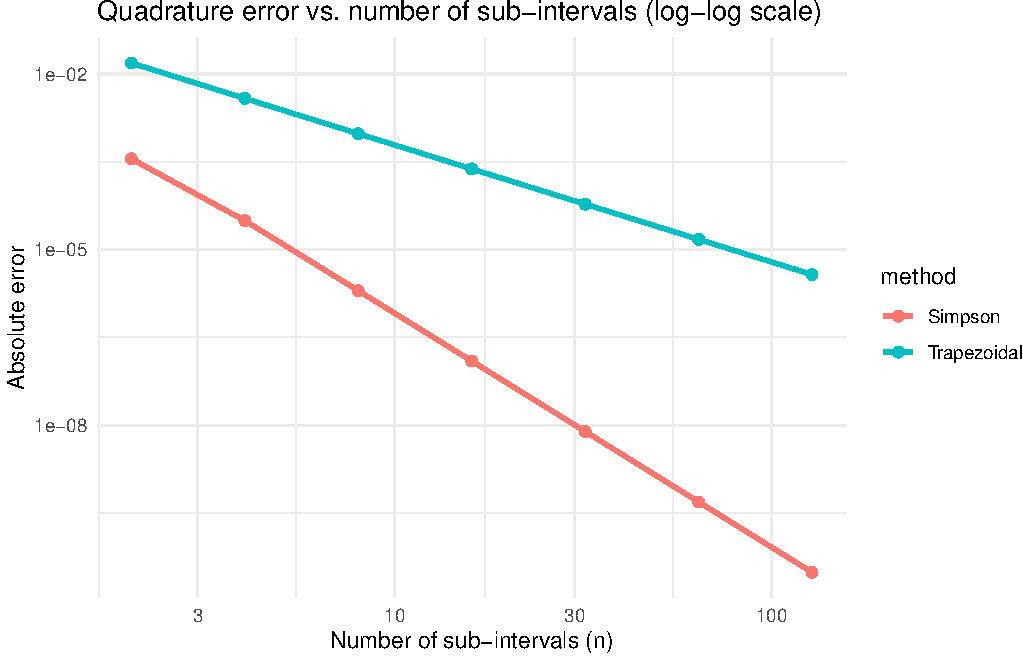
\includegraphics{04-02_Numerical_Methods_files/figure-latex/log-log-convergence-plot-1} 

}

\caption{Log-log plot of quadrature error against number of sub-intervals: the trapezoidal rule's slope of -2 and Simpson's rule's slope of -4 confirm the O(h^2) and O(h^4) rates of Section 8.}\label{fig:log-log-convergence-plot}
\end{figure}

\begin{Shaded}
\begin{Highlighting}[]
\NormalTok{x\_grid\_plot }\OtherTok{\textless{}{-}} \FunctionTok{seq}\NormalTok{(}\DecValTok{1}\NormalTok{, }\DecValTok{2}\NormalTok{, }\AttributeTok{length.out =} \DecValTok{200}\NormalTok{)}

\FunctionTok{ggplot}\NormalTok{() }\SpecialCharTok{+}
  \FunctionTok{geom\_line}\NormalTok{(}\AttributeTok{data =} \FunctionTok{tibble}\NormalTok{(}\AttributeTok{x =}\NormalTok{ x\_grid\_plot, }\AttributeTok{y =} \FunctionTok{target\_f}\NormalTok{(x\_grid\_plot)), }\FunctionTok{aes}\NormalTok{(x, y), }\AttributeTok{colour =} \StringTok{"steelblue"}\NormalTok{) }\SpecialCharTok{+}
  \FunctionTok{geom\_hline}\NormalTok{(}\AttributeTok{yintercept =} \DecValTok{0}\NormalTok{, }\AttributeTok{colour =} \StringTok{"grey60"}\NormalTok{) }\SpecialCharTok{+}
  \FunctionTok{geom\_point}\NormalTok{(}
    \AttributeTok{data =} \FunctionTok{tibble}\NormalTok{(}\AttributeTok{x =}\NormalTok{ newton\_result}\SpecialCharTok{$}\NormalTok{history, }\AttributeTok{y =} \FunctionTok{target\_f}\NormalTok{(newton\_result}\SpecialCharTok{$}\NormalTok{history)),}
    \FunctionTok{aes}\NormalTok{(x, y), }\AttributeTok{colour =} \StringTok{"darkred"}\NormalTok{, }\AttributeTok{size =} \DecValTok{2}
\NormalTok{  ) }\SpecialCharTok{+}
  \FunctionTok{geom\_path}\NormalTok{(}
    \AttributeTok{data =} \FunctionTok{tibble}\NormalTok{(}\AttributeTok{x =}\NormalTok{ newton\_result}\SpecialCharTok{$}\NormalTok{history, }\AttributeTok{y =} \FunctionTok{target\_f}\NormalTok{(newton\_result}\SpecialCharTok{$}\NormalTok{history)),}
    \FunctionTok{aes}\NormalTok{(x, y), }\AttributeTok{colour =} \StringTok{"darkred"}\NormalTok{, }\AttributeTok{linetype =} \StringTok{"dotted"}
\NormalTok{  ) }\SpecialCharTok{+}
  \FunctionTok{labs}\NormalTok{(}\AttributeTok{title =} \StringTok{"Newton{-}Raphson iterates on f(x) = x\^{}3 {-} x {-} 2"}\NormalTok{, }\AttributeTok{x =} \StringTok{"x"}\NormalTok{, }\AttributeTok{y =} \StringTok{"f(x)"}\NormalTok{) }\SpecialCharTok{+}
  \FunctionTok{theme\_minimal}\NormalTok{(}\AttributeTok{base\_size =} \DecValTok{11}\NormalTok{)}
\end{Highlighting}
\end{Shaded}

\begin{figure}

{\centering 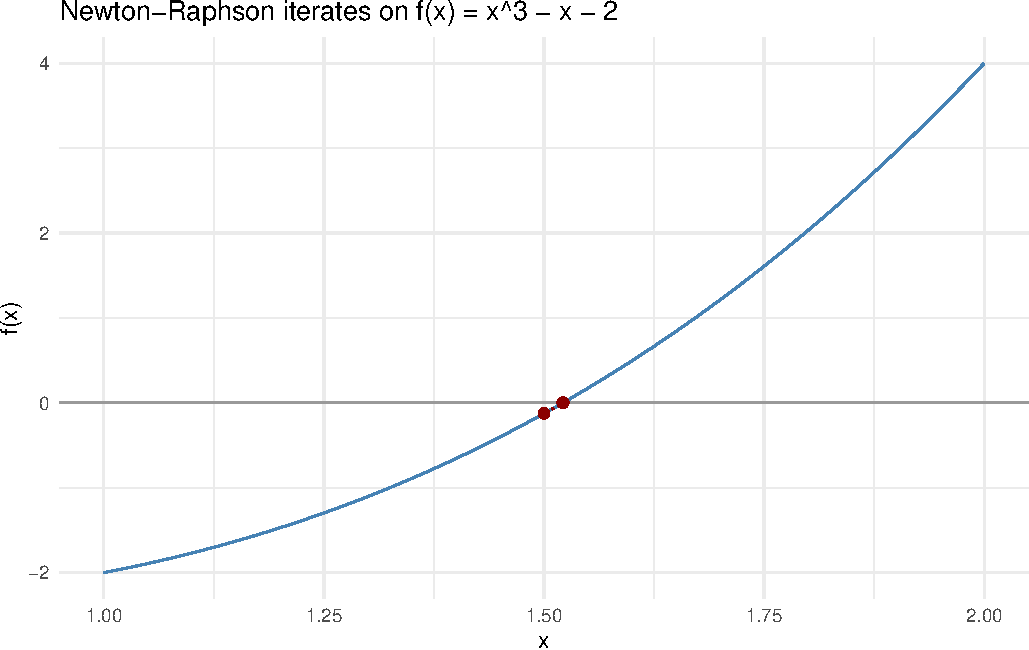
\includegraphics{04-02_Numerical_Methods_files/figure-latex/newton_basin_plot-1} 

}

\caption{Newton-Raphson iterates converge quadratically to the true root, visualized against the target function.}\label{fig:newton_basin_plot}
\end{figure}

\section{Numerical Examples}\label{numerical-examples}

\textbf{Example 1: Bisection method.}

\emph{Problem.} Find a root of \(f(x)=x^3-x-2\) in \([1,2]\), performing
three iterations of bisection by hand.

\emph{Solution.} \(f(1)=-2\), \(f(2)=4\) (opposite signs, bracket
valid).

\[
\begin{aligned}
c_1 &= 1.5, & f(1.5) &= -0.125 \ (\text{same sign as } f(1)) \Rightarrow \text{new bracket } [1.5,2] \\
c_2 &= 1.75, & f(1.75) &= 1.609375 \ (\text{opposite sign}) \Rightarrow \text{new bracket } [1.5,1.75] \\
c_3 &= 1.625, & f(1.625) &= 0.666016 \ (\text{opposite sign}) \Rightarrow \text{new bracket } [1.5,1.625]
\end{aligned}
\]

\emph{Interpretation.} After three iterations the bracket has shrunk
from width \(1\) to width \(0.125 = 1/8\), exactly matching the halving
predicted by Theorem 2.1; the true root, \(r\approx1.521380\), indeed
lies in \([1.5,1.625]\).

\textbf{Example 2: Newton-Raphson method.}

\emph{Problem.} Using the same \(f\), with \(f'(x)=3x^2-1\), perform two
iterations of Newton-Raphson from \(x_0=1.5\).

\emph{Solution.}

\[
x_1 = 1.5 - \frac{f(1.5)}{f'(1.5)} = 1.5 - \frac{-0.125}{5.75} = 1.521739,
\]

\[
x_2 = x_1 - \frac{f(x_1)}{f'(x_1)} = 1.521739 - \frac{0.002137}{5.94707} = 1.521380.
\]

\emph{Interpretation.} Two Newton-Raphson iterations already match the
true root \(r=1.521380\) to six decimal places, whereas three bisection
iterations (Example 1) had only localized the root to the interval
\([1.5,1.625]\) --- a striking illustration of the practical difference
between linear and quadratic convergence.

\textbf{Example 3: Newton-Raphson for a system.}

\emph{Problem.} Solve \(x^2+y^2=4\), \(xy=1\) starting from
\((x_0,y_0)=(1.8,0.6)\), performing one iteration by hand.

\emph{Solution.}
\(\mathbf F(1.8,0.6) = (1.8^2+0.6^2-4,\ 1.8\times0.6-1) =
(-0.4,\ 0.08)\). The Jacobian is
\(J = \begin{pmatrix}2x&2y\\y&x\end{pmatrix}\), so
\(J(1.8,0.6)=\begin{pmatrix}3.6&1.2\\0.6&1.8\end{pmatrix}\), with
determinant \(3.6(1.8)-1.2(0.6)=5.76\). Solving
\(J\boldsymbol\delta=-\mathbf F\),

\[
\boldsymbol\delta = \frac{1}{5.76}\begin{pmatrix}1.8&-1.2\\-0.6&3.6\end{pmatrix}
\begin{pmatrix}0.4\\-0.08\end{pmatrix}
= \frac{1}{5.76}\begin{pmatrix}0.816\\-0.528\end{pmatrix}
= \begin{pmatrix}0.141667\\-0.091667\end{pmatrix},
\]

so
\((x_1,y_1) = (1.8+0.141667,\ 0.6-0.091667) = (1.941667,\ 0.508333)\).

\emph{Interpretation.} Checking, \(x_1^2+y_1^2=4.0285\) and
\(x_1y_1=0.9870\), both markedly closer to the target values \(4\) and
\(1\) than the starting point; further iterations converge quadratically
to the true solution
\((\sqrt{2+\sqrt3},\ 1/\sqrt{2+\sqrt3}) \approx (1.931852,\
0.517638)\).

\textbf{Example 4: Trapezoidal and Simpson's rule.}

\emph{Problem.} Approximate \(\int_0^2 x^2\,dx\) (true value
\(8/3=2.666667\)) using \(n=4\) sub-intervals (\(h=0.5\)) with both
rules.

\emph{Solution.} Nodes: \(0, 0.5, 1, 1.5, 2\) with values
\(0, 0.25, 1, 2.25,
4\).

\[
T = \frac{0.5}{2}\bigl[0+2(0.25+1+2.25)+4\bigr] = 0.25(11) = 2.75.
\]

\[
S = \frac{0.5}{3}\bigl[0+4(0.25)+2(1)+4(2.25)+4\bigr]
= \frac{0.5}{3}(16) = 2.666667.
\]

\emph{Interpretation.} Simpson's rule reproduces the true value
\emph{exactly}, because \(f(x)=x^2\) is a polynomial of degree \(2<4\)
and Simpson's rule has degree of precision \(3\) (it integrates every
cubic exactly, hence certainly every quadratic); the trapezoidal rule,
exact only for linear integrands, overestimates the true value by
\(0.0833\), consistent with the error formula (2.8), since
\(f''(x)=2>0\) makes the trapezoidal rule systematically overestimate a
convex function.

\section{Applications}\label{applications}

\begin{itemize}
\tightlist
\item
  \textbf{Statistics.} Newton-Raphson (or its close relative, Fisher
  scoring) solves the score equations of maximum likelihood estimation
  for logistic regression, Poisson regression, and virtually every
  generalized linear model fit by standard software.
\item
  \textbf{Machine Learning.} Newton's method and its quasi-Newton
  variants (BFGS, L-BFGS) are core second-order optimization algorithms;
  the Newton-Raphson system update (2.5) is precisely the Newton step
  used in optimizing a smooth loss function, applied to its gradient.
\item
  \textbf{Data Science.} Numerical integration is used to compute
  marginal densities, expectations, and normalizing constants of fitted
  probability models that lack closed-form integrals.
\item
  \textbf{Finance.} Computing implied volatility from an option's market
  price is a classical one-dimensional root-finding problem, almost
  universally solved by Newton-Raphson or a safeguarded bisection
  hybrid.
\item
  \textbf{Reliability Engineering.} Solving for a system's failure time
  or reliability threshold from a nonlinear hazard or reliability
  function often requires root-finding when no closed-form inverse
  exists.
\item
  \textbf{Monte Carlo Methods.} Numerical quadrature provides the
  deterministic benchmark against which the Monte Carlo integration
  methods of Unit 4.3 are compared for low-dimensional integrals.
\item
  \textbf{Bayesian Statistics.} The Laplace approximation to a posterior
  density requires locating the posterior mode via Newton-Raphson (or a
  quasi-Newton method) and evaluating the Hessian there.
\item
  \textbf{Operations Research.} Root-finding is used to solve for
  equilibrium points or break-even conditions in nonlinear resource
  allocation and inventory models.
\item
  \textbf{Engineering.} Newton-Raphson for systems is the standard
  method for solving the nonlinear equilibrium equations arising in
  structural and circuit analysis.
\end{itemize}

\section{Advantages}\label{advantages}

\begin{itemize}
\tightlist
\item
  Bisection is completely robust: given a valid bracket, it is
  mathematically guaranteed to converge, requiring only continuity of
  \(f\).
\item
  Newton-Raphson converges very rapidly (quadratically) once near a
  simple root, needing very few iterations for high precision.
\item
  Simpson's rule achieves a substantially higher order of accuracy than
  the trapezoidal rule at essentially the same computational cost per
  additional node.
\end{itemize}

\section{Limitations}\label{limitations}

\begin{itemize}
\tightlist
\item
  Bisection requires an initial bracket with a sign change, which may
  not always be easy to locate, particularly for functions with multiple
  close roots or no sign change at a simple root (a root of even
  multiplicity).
\item
  Newton-Raphson requires the derivative \(f'\) (or the Jacobian, for
  systems), can diverge or converge to an unintended root from a poor
  starting point, and can fail outright if \(f'(x_n)\) is ever zero or
  numerically close to it during the iteration.
\item
  Fixed-\(n\) quadrature rules such as trapezoidal and Simpson's rules
  degrade sharply for integrands with singularities, sharp peaks, or
  discontinuities, and provide no built-in error estimate without
  additional (e.g.~Richardson extrapolation) machinery.
\end{itemize}

\section{Practical Tips}\label{practical-tips}

\begin{itemize}
\tightlist
\item
  \textbf{Prefer a hybrid strategy in production code.} Combining
  Newton-Raphson's speed with bisection's robustness (falling back to a
  bisection step whenever a Newton step would leave the current bracket)
  is standard practice, as implemented internally by professional
  root-finders including R's \texttt{uniroot()}.
\item
  \textbf{Always verify convergence, not just iteration count.} Checking
  both \(|x_{n+1}-x_n|\) and \(|f(x_{n+1})|\) against separate
  tolerances guards against premature termination when the two
  quantities behave differently (as can happen near a root with a very
  flat or very steep derivative).
\item
  \textbf{Use Simpson's rule by default over the trapezoidal rule} for
  smooth integrands, since it is essentially free --- the same number of
  function evaluations yields two additional orders of accuracy.
\item
  \textbf{Use \texttt{integrate()}'s adaptive quadrature, not a
  fixed-\(n\) composite rule, for integrands with peaks or
  singularities.} Fixed-node rules waste evaluations on flat regions and
  under-resolve rapidly varying regions.
\item
  \textbf{When implementing Newton-Raphson for systems, monitor the
  condition number of the Jacobian.} A poorly conditioned or singular
  Jacobian at any iterate is a common, silent cause of numerical failure
  that a simple convergence check may not reveal until many wasted
  iterations have passed.
\end{itemize}

\section{Summary}\label{summary}

\begin{itemize}
\tightlist
\item
  The bisection method locates a root by repeatedly halving a bracket
  known to contain a sign change; Theorem 2.1 establishes its
  unconditional linear convergence.
\item
  The Newton-Raphson method follows the tangent line to a root and, near
  a simple root, converges quadratically (Theorem 2.2), roughly doubling
  the number of correct digits per iteration.
\item
  Newton-Raphson generalizes to systems of nonlinear equations via the
  Jacobian matrix, replacing division by \(f'\) with solving a linear
  system involving \(J\).
\item
  The trapezoidal and Simpson's rules approximate a definite integral
  using linear and quadratic local interpolation respectively, with
  error terms \(O(h^2)\) and \(O(h^4)\) derived explicitly in Section 8,
  and verified empirically by the log-log convergence plot of Section

  \begin{enumerate}
  \def\labelenumi{\arabic{enumi}.}
  \setcounter{enumi}{9}
  \tightlist
  \item
  \end{enumerate}
\item
  These deterministic numerical methods underlie the practical
  computation of maximum likelihood estimates and intractable integrals
  throughout statistical computing.
\end{itemize}

\section{Key Formulae}\label{key-formulae}

\begin{itemize}
\tightlist
\item
  Bisection error bound: \(|c_k-r| \le (b_0-a_0)/2^{k+1}\).
\item
  Newton-Raphson update: \(x_{n+1}=x_n - f(x_n)/f'(x_n)\); quadratic
  error recursion \(e_{n+1} = -\dfrac{f''(\xi_n)}{2f'(x_n)}e_n^2\).
\item
  Newton-Raphson for systems: \(\mathbf x_{n+1} = \mathbf x_n -
  J(\mathbf x_n)^{-1}\mathbf F(\mathbf x_n)\).
\item
  Trapezoidal rule: \(T=\dfrac{h}{2}[f(x_0)+2\sum f(x_i)+f(x_n)]\),
  error \(-\dfrac{(b-a)h^2}{12}f''(\xi)\).
\item
  Simpson's rule: \(S=\dfrac{h}{3}[f(x_0)+4\sum_{\text{odd}}f(x_i)
  +2\sum_{\text{even}}f(x_i)+f(x_n)]\), error
  \(-\dfrac{(b-a)h^4}{180}f''''(\xi)\).
\end{itemize}

\section{Key Terms}\label{key-terms}

\begin{itemize}
\tightlist
\item
  \textbf{Bisection method.} A bracketing root-finding method that
  repeatedly halves an interval known to contain a sign change.
\item
  \textbf{Bracket.} An interval on which a continuous function changes
  sign, guaranteeing a root within it.
\item
  \textbf{Degree of precision.} The highest polynomial degree a
  quadrature rule integrates exactly.
\item
  \textbf{Jacobian matrix.} The matrix of first partial derivatives of a
  vector-valued function.
\item
  \textbf{Newton-Raphson method.} A root-finding method that follows the
  tangent line (or hyperplane) at the current iterate to a new estimate.
\item
  \textbf{Quadratic convergence.} A convergence rate in which the error
  at each step is proportional to the square of the previous error.
\item
  \textbf{Simpson's rule.} A quadrature formula based on local quadratic
  (parabolic) interpolation.
\item
  \textbf{Trapezoidal rule.} A quadrature formula based on local linear
  interpolation.
\end{itemize}

\section{Exercises}\label{exercises}

\subsection{Multiple Choice Questions}\label{multiple-choice-questions}

\begin{enumerate}
\def\labelenumi{\arabic{enumi}.}
\tightlist
\item
  The bisection method requires

  \begin{enumerate}
  \def\labelenumii{(\alph{enumii})}
  \tightlist
  \item
    a derivative of \(f\)
  \item
    a bracket \([a,b]\) with \(f(a)f(b)<0\)
  \item
    a Hessian matrix
  \item
    a Taylor series expansion
  \end{enumerate}
\item
  The bisection method's convergence rate is

  \begin{enumerate}
  \def\labelenumii{(\alph{enumii})}
  \tightlist
  \item
    quadratic
  \item
    cubic
  \item
    linear
  \item
    exponential
  \end{enumerate}
\item
  The Newton-Raphson update formula is

  \begin{enumerate}
  \def\labelenumii{(\alph{enumii})}
  \tightlist
  \item
    \(x_{n+1}=x_n+f(x_n)/f'(x_n)\)
  \item
    \(x_{n+1}=x_n-f(x_n)/f'(x_n)\)
  \item
    \(x_{n+1}=x_n-f'(x_n)/f(x_n)\)
  \item
    \(x_{n+1}=x_n-f(x_n)f'(x_n)\)
  \end{enumerate}
\item
  Newton-Raphson achieves quadratic convergence provided

  \begin{enumerate}
  \def\labelenumii{(\alph{enumii})}
  \tightlist
  \item
    \(f\) is continuous only
  \item
    the root is simple and \(f''\) is continuous nearby
  \item
    \(f\) is a polynomial of even degree
  \item
    the starting point is exactly the root
  \end{enumerate}
\item
  The Newton-Raphson update for a system of equations replaces division
  by \(f'\) with

  \begin{enumerate}
  \def\labelenumii{(\alph{enumii})}
  \tightlist
  \item
    multiplication by \(J\)
  \item
    solving a linear system involving the Jacobian \(J\)
  \item
    computing eigenvalues of \(J\)
  \item
    transposing \(J\)
  \end{enumerate}
\item
  The trapezoidal rule's composite error is of order

  \begin{enumerate}
  \def\labelenumii{(\alph{enumii})}
  \tightlist
  \item
    \(O(h)\)
  \item
    \(O(h^2)\)
  \item
    \(O(h^3)\)
  \item
    \(O(h^4)\)
  \end{enumerate}
\item
  Simpson's rule's composite error is of order

  \begin{enumerate}
  \def\labelenumii{(\alph{enumii})}
  \tightlist
  \item
    \(O(h^2)\)
  \item
    \(O(h^3)\)
  \item
    \(O(h^4)\)
  \item
    \(O(h^5)\)
  \end{enumerate}
\item
  Simpson's rule requires

  \begin{enumerate}
  \def\labelenumii{(\alph{enumii})}
  \tightlist
  \item
    an odd number of sub-intervals
  \item
    an even number of sub-intervals
  \item
    exactly 2 sub-intervals
  \item
    no restriction on the number of sub-intervals
  \end{enumerate}
\item
  Simpson's rule integrates every polynomial of degree up to

  \begin{enumerate}
  \def\labelenumii{(\alph{enumii})}
  \tightlist
  \item
    1
  \item
    2
  \item
    3
  \item
    4
  \end{enumerate}
\item
  A common safeguard against Newton-Raphson divergence is to

  \begin{enumerate}
  \def\labelenumii{(\alph{enumii})}
  \tightlist
  \item
    always start at \(x_0=0\)
  \item
    combine it with a bisection fallback
  \item
    use only the trapezoidal rule instead
  \item
    increase the tolerance to a very large value
  \end{enumerate}
\end{enumerate}

\textbf{Answers.} 1(b), 2(c), 3(b), 4(b), 5(b), 6(b), 7(c), 8(b), 9(c),
10(b).

\subsection{Short Answer Questions}\label{short-answer-questions}

\begin{enumerate}
\def\labelenumi{\arabic{enumi}.}
\tightlist
\item
  State the bracketing condition required to start the bisection method,
  and explain why it guarantees a root exists.
\item
  Explain, in one or two sentences, the geometric idea behind the
  Newton-Raphson method.
\item
  Write the multivariate Newton-Raphson update formula and identify the
  role of the Jacobian matrix.
\item
  State the error order of the trapezoidal rule and of Simpson's rule,
  and explain which is more accurate for the same \(n\).
\item
  Explain why Simpson's rule requires an even number of sub-intervals.
\item
  Why can Newton-Raphson fail even when a root exists nearby?
\item
  Explain the difference between linear and quadratic convergence in
  terms of the number of correct digits gained per iteration.
\item
  Why is bisection often used as a fallback for Newton-Raphson in
  production software?
\item
  Give one statistical application of Newton-Raphson distinct from those
  emphasized in this unit.
\item
  Explain why Simpson's rule integrates \(x^2\) exactly, as verified in
  Example 4.
\end{enumerate}

\subsection{Long Answer Questions}\label{long-answer-questions}

\begin{enumerate}
\def\labelenumi{\arabic{enumi}.}
\tightlist
\item
  State and prove Theorem 2.1 (linear convergence of bisection).
\item
  State and prove Theorem 2.2 (quadratic convergence of Newton-Raphson),
  explaining the role of Taylor's theorem in the proof.
\item
  Derive the composite trapezoidal rule error formula, showing every
  step from the linear interpolation error to the final composite bound.
\item
  Derive the single-panel Simpson's rule error formula using the Taylor
  expansion approach of Section 8.2, showing every algebraic step.
\item
  Compare bisection and Newton-Raphson in terms of robustness, speed,
  and information required about \(f\), and describe a scenario in which
  each would be preferred.
\item
  Derive the Newton-Raphson update formula for a system of two nonlinear
  equations from the first-order Taylor expansion of \(\mathbf F\),
  explaining each step.
\item
  Discuss the role of Newton-Raphson (or Fisher scoring) in maximum
  likelihood estimation, explaining how the score equation and the
  observed or expected information relate to \(f\) and \(f'\) in the
  scalar case.
\item
  Explain why fixed-\(n\) trapezoidal and Simpson's rules can perform
  poorly for integrands with sharp peaks or singularities, and describe
  how adaptive quadrature addresses this limitation.
\item
  Using the numerical example of Section 11 (Example 4), explain why the
  trapezoidal rule systematically overestimates the integral of a convex
  function, relating your answer to the sign of the error term (2.8).
\item
  Discuss the practical safeguards used in professional root-finding
  software to combine the reliability of bisection with the speed of
  Newton-Raphson.
\end{enumerate}

\subsection{Programming Exercises}\label{programming-exercises}

\begin{enumerate}
\def\labelenumi{\arabic{enumi}.}
\tightlist
\item
  Implement \texttt{bisection\_method()} and
  \texttt{newton\_raphson\_method()} from first principles (already
  provided) and reproduce the manual iterations of Examples 1 and 2
  exactly.
\item
  Implement \texttt{newton\_raphson\_system()} from first principles
  (already provided) and verify the manual first iteration of Example 3,
  then run the algorithm to convergence and confirm it reaches the true
  solution given in the interpretation of that example.
\item
  Implement \texttt{trapezoidal\_rule()} and \texttt{simpsons\_rule()}
  from first principles (already provided) and reproduce the manual
  calculation of Example 4 exactly.
\item
  Reproduce the log-log convergence plot of Section 10 for a different
  smooth integrand of your choosing, and verify the fitted slopes are
  close to \(-2\) (trapezoidal) and \(-4\) (Simpson).
\item
  Use Newton-Raphson to compute the maximum likelihood estimate of the
  rate parameter of an Exponential distribution from simulated data, and
  verify your answer against the known closed-form MLE \(1/\bar x\).
\item
  Use \texttt{newton\_raphson\_system()} to fit, by maximum likelihood,
  the two parameters of a simple two-parameter distribution of your
  choosing (for example, a Gamma distribution) to simulated data,
  comparing your result to R's built-in \texttt{optim()} or
  \texttt{fitdistr()}.
\item
  Write a function that applies Newton-Raphson to invert the standard
  Normal cumulative distribution function (i.e.~compute \(\Phi^{-1}(u)\)
  without using \texttt{qnorm()}), and compare its output and speed to
  \texttt{qnorm()} for a range of \(u\) values.
\item
  Investigate Newton-Raphson divergence empirically: for
  \(f(x)=x^3-2x+2\), show that starting from \(x_0=0\) causes the
  iteration to cycle indefinitely, while starting from \(x_0=-2\)
  converges; explain the difference using a plot of \(f\) and its
  tangent lines.
\item
  Implement Richardson extrapolation for the trapezoidal rule (combining
  the estimates at \(n\) and \(2n\) sub-intervals to cancel the leading
  error term) and verify empirically that it achieves an error order
  comparable to Simpson's rule.
\item
  Write a function comparing the number of function evaluations required
  by bisection, Newton-Raphson, and R's built-in \texttt{uniroot()} to
  reach a fixed tolerance for a common test function, and tabulate the
  results.
\end{enumerate}

\subsection{Mini Projects}\label{mini-projects}

\begin{enumerate}
\def\labelenumi{\arabic{enumi}.}
\item
  \textbf{A robust hybrid root-finder.} Implement a root-finding
  function that combines bisection and Newton-Raphson: at each step,
  attempt a Newton-Raphson update, but fall back to a bisection step
  whenever the Newton step would leave the current bracket or the
  derivative is too close to zero. Test your hybrid method against plain
  Newton-Raphson on at least three test functions chosen to make plain
  Newton-Raphson struggle (for example, functions with nearby inflection
  points or very flat derivatives near the root), and report the
  iteration counts and reliability of each approach.
\item
  \textbf{Numerical integration for a Bayesian normalizing constant.}
  Consider a posterior density known only up to a normalizing constant,
  \(\pi(\theta) \propto L(\theta)\,p(\theta)\), for a likelihood \(L\)
  and prior \(p\) of your choosing (for a single parameter \(\theta\)).
  Use the composite Simpson's rule to compute the normalizing constant
  \(\int \pi(\theta)\,d\theta\) over a suitable range, verify
  convergence of your answer as \(n\) increases, and use the normalized
  posterior to compute the posterior mean via a second application of
  Simpson's rule. Compare your results to a Monte Carlo integration
  estimate (a preview of Unit 4.3).
\end{enumerate}

\textbf{Difficulty labels.} Multiple choice, short answer:
\textbf{Easy}. Long answer questions 3, 4, 6, 8, 9, programming
exercises 1-6: \textbf{Medium}. Long answer questions 1, 2, 5, 7, 10,
programming exercises 7-10: \textbf{Medium to Advanced}. Mini projects:
\textbf{Advanced}.

\section{References}\label{references}

Burden, R. L., \& Faires, J. D. (2011). \emph{Numerical analysis} (9th
ed.). Brooks/Cole.

Kelley, C. T. (2003). \emph{Solving nonlinear equations with Newton's
method}. SIAM.

Nocedal, J., \& Wright, S. J. (2006). \emph{Numerical optimization} (2nd
ed.). Springer.

Rizzo, M. L. (2019). \emph{Statistical computing with R} (2nd ed.). CRC
Press.

Ross, S. M. (2020). \emph{Simulation} (6th ed.). Academic Press.

\end{document}
